\graphicspath{{chapters/ch-introduction/figures/}}
\chapter{Introduction}


\label{sec:introduction}

Until now, research in the sensor network domain has mainly focused on
routing, data aggregation, and energy conservation inside a single
sensor network while the integration of multiple sensor networks has
only been studied to a limited extent. However, as the price of
wireless sensors diminishes rapidly we can soon expect large numbers
of autonomous sensor networks being deployed. These sensor networks
will be managed by different organizations but the interconnection of
their infrastructures along with data integration and distributed
query processing will soon become an issue to fully exploit the
potential of this ``Sensor Internet.'' This requires platforms which
enable the dynamic integration and management of sensor networks and
the produced data streams.

The Global Sensor Networks (GSN) platform aims at providing a flexible
middleware to accomplish these goals.  GSN assumes the simple model
shown in Figure~\ref{fig:setup}. A sensor network internally may use
arbitrary multi-hop, ad-hoc routing algorithms to deliver sensor
readings to one or more sink node(s). A sink node is a node which is
connected to a more powerful base computer which in turn runs the GSN
middleware and may participate in a (large-scale) network of base
computers, each running GSN and servicing one or more sensor networks.

\begin{figure}
  \centering
  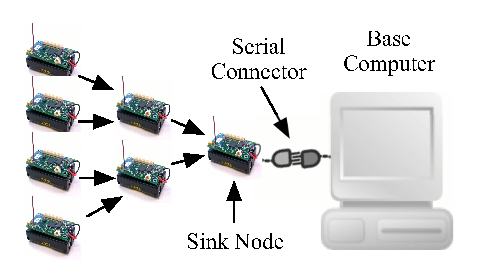
\includegraphics[width=0.5\columnwidth]{model}
  \caption{GSN model}
  \label{fig:setup}
\end{figure}

We do not make any assumptions on the internals of a sensor network
other than that the sink node is connected to the base computer via a
software wrapper conforming to the GSN API. On top of this physical
access layer GSN provides so-called \textit{virtual sensors} which
abstract from implementation details of access to sensor data and
define the data stream processing to be performed. Local and remote
virtual sensors, their data streams and the associated query
processing can be combined in arbitrary ways and thus enable the user
to build a data-oriented ``Sensor Internet'' consisting of sensor
networks connected via GSN.

\begin{comment} %following paragraph not really relevant in this context
In the following we start with a detailed description of the virtual
sensor abstraction in Section~\ref{sec:virt-sens-spec}, discuss GSN's
data stream processing and time model in
Section~\ref{sec:data-stre-proc}, and present GSN's system architecture
along with a discussion of essential implementation details
in Section~\ref{sec:system-architecture}. We
evaluate the performance of GSN in Section~\ref{sec:evaluation} and
discuss related work in Section~\ref{sec:relatedwork} before
concluding.
\end{comment}
\section{Terminology}

\begin{itemize}
	\item \textbf{Global Sensor Networks} (\gsn) defines both the project and the software described in this document. \\
	\item A \textbf{Wrapper} (\wrapper) is a piece of Java code that does the data acquisition for a specific type of device. \\
	\item A \textbf{Virtual Sensor} (\vs) is the main component in \gsn. It receives data from one or more \wrapper. It can combine their data, 
		process and finally store it. A \vs is defined in a single \vsd and combines different pieces of software 
	\begin{itemize}
		\item One \vsp
		\item Zero or Many \wrapper\textit{(s)}
	\end{itemize}
	\item A \textbf{Virtual Sensor Description file} (\vsd) is an XML file that contains the selection and the parametrization of the \vsp and \wrapper that compose a \vs.
		This file also contains the SQL statements that connect them together. \\
	\item A \textbf{Virtual Sensor Processing class} (\vsp) is a piece of Java code that process and stores the data upon reception from the \wrapper. \\
\end{itemize}

\section{Quick Start}

GSN (for Global Sensor Networks) is a software project that started in
2005 at EPFL in the LSIR Lab by Ali Salehi, under the supervision of
Prof. Karl Aberer. The initial goal was to provide a reusable software
platform for the processing of data streams generated by wireless
sensor networks. The project was successful, and was later reoriented
towards a generic stream processing platform.

GSN acquires data, filters it with an intuitive, enriched SQL syntax,
runs customisable algorithms on the results of the query, and outputs
the generated data with its notification subsystem.

GSN can be configured to acquire data from various data sources. The
high number of data sources in GSN allows for sophisticated data
processing scenarios. In the unlikely event that your data sources are
not supported, it is very easy to write a wrapper to make your hardware
work with GSN (you can find more information about this in chapter 5).

GSN offers advanced data filtering functionalities through an enhanced
SQL syntax. It is assumed that the reader has some knowledge of the
Standard Query Language (SQL). Using it for basic operations is fairly
intuitive and you should be able to start using it from the examples
provided in this document.
